\documentclass[border=3pt]{standalone}
% Shared TikZ styles for the Ch. 3–8 diagrams (standalone PDFs); extends the Ch. 1 palette (s1_vs_llm_common.tex).
\usepackage[T1]{fontenc}
\usepackage{lmodern}
\usepackage[english]{babel}
\usepackage{amsmath,amssymb}
\usepackage{tikz}
\usetikzlibrary{shapes.geometric,shapes.misc,positioning,fit,arrows.meta,calc,backgrounds,decorations.pathreplacing,patterns}
\definecolor{ioFill}{HTML}{F1F0EC}\definecolor{ioLine}{HTML}{52514E}
\definecolor{modFill}{HTML}{E8F1FB}\definecolor{modLine}{HTML}{2A78D6}
\definecolor{decFill}{HTML}{ECE9F7}\definecolor{decLine}{HTML}{4A3AA7}
\definecolor{postFill}{HTML}{FFF6E0}\definecolor{postLine}{HTML}{EDA100}
\definecolor{okFill}{HTML}{EAF7F1}\definecolor{okLine}{HTML}{1BAF7A}
\definecolor{badFill}{HTML}{FDECEC}\definecolor{badLine}{HTML}{E34948}
\definecolor{nmFill}{HTML}{EFEAF8}\definecolor{nmLine}{HTML}{4A3AA7}
\definecolor{loopRed}{HTML}{E34948}\definecolor{clusterLine}{HTML}{9A9890}\definecolor{ink2}{HTML}{52514E}
\definecolor{orangeA}{HTML}{EB6834}
\tikzset{
  every node/.style={font=\small, align=center},
  io/.style={trapezium, trapezium left angle=72, trapezium right angle=108, trapezium stretches body,
             draw=ioLine, fill=ioFill, thick, inner sep=3pt, minimum height=2.4em},
  model/.style={rectangle, draw=modLine, fill=modFill, very thick, inner sep=4pt, minimum height=2.4em, text width=#1},
  model/.default=3.6cm,
  post/.style={rectangle, draw=postLine, fill=postFill, very thick, inner sep=4pt, minimum height=2.2em, text width=#1},
  post/.default=3.6cm,
  data/.style={cylinder, shape border rotate=90, aspect=0.18, draw=okLine, fill=okFill, very thick, inner sep=3pt, minimum height=2.6em, text width=#1},
  data/.default=2.4cm,
  decision/.style={diamond, aspect=2.1, draw=decLine, fill=decFill, very thick, inner sep=1pt},
  outcome/.style={rounded rectangle, draw=#1, thick, inner sep=4pt, minimum height=2em},
  arrow/.style={-{Latex[length=2mm]}, thick, ioLine},
  dashedarrow/.style={-{Latex[length=2mm]}, thick, ioLine, dashed},
  loop/.style={-{Latex[length=2.4mm]}, line width=1.4pt, loopRed},
  cluster/.style={draw=clusterLine, dashed, rounded corners=3pt, inner sep=7pt},
  clusterlabel/.style={font=\small\bfseries, text=ioLine},
  note/.style={font=\footnotesize, text=ink2},
  tok/.style={rectangle, draw=ioLine, fill=ioFill, thin, inner sep=2pt, minimum height=1.6em, font=\footnotesize},
  vmark/.style={rectangle, draw=orangeA, fill=postFill, thick, inner sep=2pt, minimum height=1.6em, font=\footnotesize\ttfamily},
}

\begin{document}
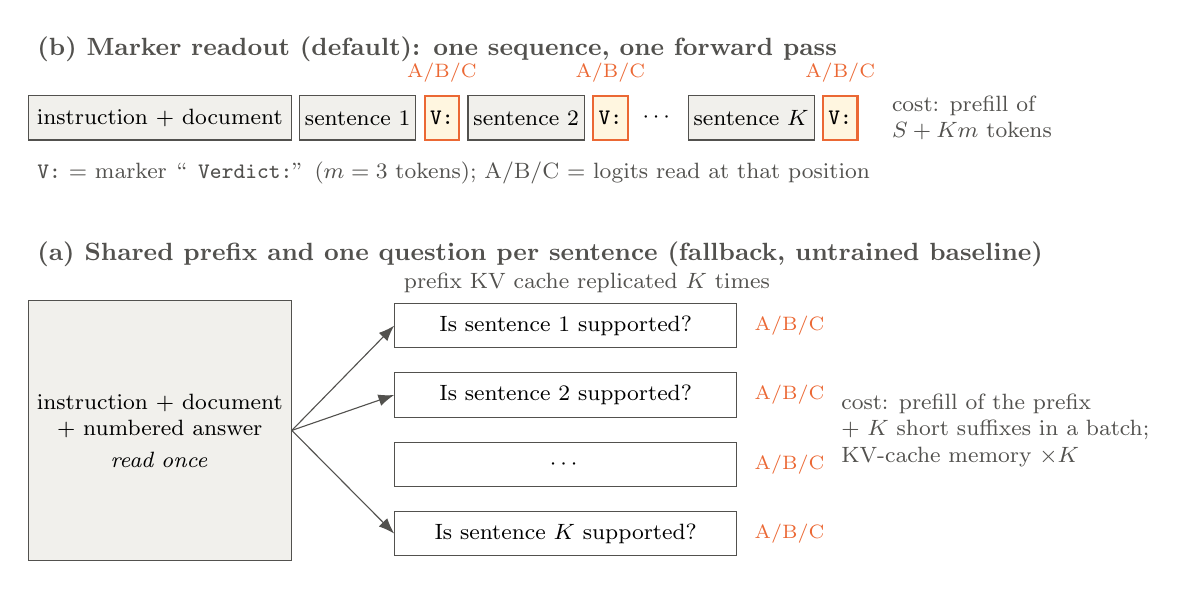
\begin{tikzpicture}[node distance=0.9mm]
  % ---------- design (b) ----------
  \node[clusterlabel, anchor=west] (tb) at (0,0) {(b) Marker readout (default): one sequence, one forward pass};
  \node[tok, text width=3.2cm, below right=3mm and 0mm of tb.south west] (pb) {instruction + document};
  \node[tok, right=of pb] (b1) {sentence 1};\node[vmark, right=of b1] (bm1) {V:};
  \node[tok, right=of bm1] (b2) {sentence 2};\node[vmark, right=of b2] (bm2) {V:};
  \node[right=0.5mm of bm2, font=\footnotesize] (bd) {$\cdots$};
  \node[tok, right=0.5mm of bd] (bk) {sentence $K$};\node[vmark, right=of bk] (bmk) {V:};
  \node[note, right=3mm of bmk, align=left] {cost: prefill of\\$S + Km$ tokens};
  \node[note, below=1.5mm of pb.south west, anchor=north west] {\texttt{V:} = marker ``\texttt{~Verdict:}'' ($m = 3$ tokens); A/B/C = logits read at that position};
  \foreach \n in {bm1,bm2,bmk} \node[font=\scriptsize, text=orangeA, above=0.3mm of \n] {A/B/C};
  % ---------- design (a) ----------
  \node[clusterlabel, anchor=west] (ta) at (0,-2.6) {(a) Shared prefix and one question per sentence (fallback, untrained baseline)};
  \node[tok, text width=3.2cm, minimum height=3.3cm, below right=3mm and 0mm of ta.south west] (pa) {instruction + document\\+ numbered answer\\[2pt]\textit{read once}};
  \foreach \i/\lab in {1/{Is sentence 1 supported?},2/{Is sentence 2 supported?},3/{$\cdots$},4/{Is sentence $K$ supported?}} {
    \node[tok, fill=white, text width=4.2cm, anchor=west] (q\i) at ([xshift=13mm, yshift={1.33cm-(\i-1)*0.88cm}]pa.east) {\lab};
    \node[font=\scriptsize, text=orangeA, right=1mm of q\i] {A/B/C};
  }
  \foreach \i in {1,2,4} \draw[arrow, thin] (pa.east) -- (q\i.west);
  \node[note, above=0mm of q1.north west, anchor=south west] {prefix KV cache replicated $K$ times};
  \node[note, align=left, anchor=west] at ([xshift=12mm]q2.east |- pa.east) {cost: prefill of the prefix\\+ $K$ short suffixes in a batch;\\KV-cache memory $\times K$};
\end{tikzpicture}
\end{document}
